%!TEX root = main.tex
Now that all unsolvable problems have been classified, we know that every problem left must have a $\mathcal{O}(n)$ complexity. In this section, we are going, for each problem, to find if its complexity is either $\Omega(n)$ (which would lead the problem to be $\Theta(n)$) either $O(log(n))$.
\section[Proving Omega(n)]{Proving $\Omega(n)$}
The \hyperref[sec:BLP]{\textbf{binary labelling problem}} classification implemented leads to show that $\Omega(n)$ hold for a lot of problems. Indeed, while some problems $\Pi$ having a global complexity are classified since $|A_\Pi|<3$, some other with $|A_\Pi| = 3$ are classified using the redundancy of their labels. In the case of $\wdd = 3, \bdd = 2$, this lead to the classification of 153 problems having a global complexity, as we will see later, there are the only ones.
\section[Proving O(log(n))]{Proving $O(log(n))$}
The following holds for $\wdd = 3, \bdd = 2$.
In the following, we are going to take the set $P$ of all problems that does not have any restrictions unclassified (the border problems between the unclassified problems and the $\Theta(n)$ problems) and show that each problem in $P$ have a complexity $\mathcal{O}(log(n))$. By definition of $P$, showing that they have a $log(n)$ upper bound will also show that every problems that have not been yet classified also are $\mathcal{O}(log(n))$ since they must be a restriction of a problem in $P$.

\subsection{Known logarithmic problems}
\subsibsection{The 3-vertex coloring}
It is known that d-vertex coloring has a complexity $\Theta(log_dn)$ on d-regular trees \cite{DBLP:journals/corr/ChangKP16}, therefore we can classify the 3-vertex coloring problem on 3-regular trees: $$W = \{AB, AC, BC\}, B =\{AAA,BBB,CCC\}$$

\subsubsection{The 3-edge coloring}
First, we know that d-edge coloring has a complexity $\mathcal{O}(log_dn)$  on d-regular trees with $d\geq 3$ \cite{DBLP:journals/corr/abs-1708-04290}.
We also know that 3-edge coloring has a complexity $\Omega(log_n)$ on 3-regular trees \cite{balliu2019locality}, we can then classify the 3-edge coloring problem on 3-regular trees: $$W = \{AA, BB, CC\}, B=\{ABC\}$$

\subsection{Logarithmic upper bound using sinkless and sourceless orientation}
We know that creating a sinkless and sourceless orientation (SSO) in a 3 regular has a $\Theta(log(n))$ complexity \cite{1}. Let's use this result to show that some 3 labelling problems have a $\mathcal{O}(log(n))$ complexity. To do that, for each problem, we will show that for any given graph with a SSO, a constant algorithm capable of solving it exists.\\
The SSO ensures that, on any 3 regular graph, a given node $u$ with a degree 3 has either:
\begin{itemize}
    \item 2 outgoing edges and 1 incoming edge
    \item 1 outgoing edge and 2 incoming edges
\end{itemize}
The former will be denoted $X$ when the latter $Y$
\subsubsection[(W = (ABC, BCC), B = (AC,BC)]{$W = \{ABC, BCC\}$, $B = \{AC, BC\}$}
\begin{itemize}
    \item We label the nodes of type $X$ with $BCC$ such that the port corresponding to the incoming edge is labelled with $B$
    \item We label the nodes of type $Y$ with $ABC$ such that the port corresponding to the outgoing edge is labelled with $C$
\end{itemize}
The white constraint is respected since there are no other configuration used for any node with a degree 3.
We can see that any oriented edge $(u,v)$ starts from a port of $u$ labelled with a $C$ and can either end on a port of $v$ labelled with $A$ or $B$, since the black constraint contains both $AC$ and $BC$ in both of these cases the configuration is valid.
\subsubsection[(W = (AAB, BBC), B = (AB,BC)]{$W = \{AAB, BBC\}$, $B = \{AB, BC\}$}


\begin{itemize}
    \item We label the nodes of type $X$ with $BBC$ such that the port corresponding to the incoming edge is labelled with $C$
    \item We label the nodes of type $Y$ with $AAB$ such that the port corresponding to the outgoing edge is labelled with $B$
\end{itemize}
The white constraint is respected since there is no other configuration used for any node with a degree 3.
We can see that any oriented edge $(u,v)$ starts from a port of $u$ labelled with a $B$ and can either end on a port of $v$ labelled with $A$ or $C$, since the black constraint contains both $BA$ and $BC$ in both of these cases the configuration is valid.



\subsection{Logarithmic upper bound using even orientation}
Again, we know that creating an even orientation (EO) in a 3 regular has a $\Theta(log(n))$ complexity \cite{1}. Let's use this result to show that some 3 labelling problems have a $\mathcal{O}(log(n))$ complexity. To do that, for each problem, we will show that for any given graph with a EO, a constant algorithm capable of solving it exists.\\
The EO ensures that, on any 3 regular graph, a given node $u$ with a degree 3 has either:
\begin{itemize}
    \item 2 outgoing edges and 1 incoming edge
    \item 0 outgoing edge and 3 incoming edges
\end{itemize}
The former will be denoted $X$ when the latter $Y$
\subsubsection[(W = (ABC, CCC), B = (AC,BC)]{$W = \{ABC, CCC\}$, $B = \{AC, BC\}$}
\begin{itemize}
    \item We label the nodes of type $X$ with $ABC$ such that the port corresponding to the incoming edge is labelled with $C$
    \item We label the nodes of type $Y$ with $CCC$
\end{itemize}
The white constraint is respected since there are no other configuration used for any node with a degree 3.
We can see that any oriented edge $(u,v)$ starts from a port of $u$ labelled with either $A$ or $B$ and ends on a port of $v$ labelled with $C$, since the black constraint contains both $AC$ and $BC$ in both of these cases the configuration is valid.

\subsubsection[(W = (X0X1X2, X3CC), B = (AC,BC)]{All the problems where : $W = \{X_0X_1X_2, X_3CC\}$, $B = \{AC, BC\}$ with $X_i \in \{A,B\}$ for $i=0,1,2,3$}
\begin{itemize}
    \item We label the nodes of type $X$ with $X_3CC$ such that the port corresponding to the incoming edge is labelled with $X_3$
    \item We label the nodes of type $Y$ with $X_0X_1X_2$
\end{itemize}
The white constraint is respected since there are no other configuration used for any node with a degree 3.
We can see that any oriented edge $(u,v)$ starts from a port of $u$ labelled with $C$ and ends on a port of $v$ labelled with either $A$ or $B$, since the black constraint contains both $CA$ and $CB$ in both of these cases the configuration is valid.


\subsection{Logarithmic upper bound using even orientation and a 3-edge coloring}
Again, we know that creating an even orientation (EO) in a 3 regular has a $\Theta(log(n))$ complexity \cite{1}, the same applies to creating a 3-edge coloring. Let's use these results to show that some 3 labelling problems have a $\mathcal{O}(log(n))$ complexity. To do that, for each problem, we will show that for any given graph with a EO, a constant algorithm capable of solving it exists.\\
The EO and the 3-edge coloring $(R,G,B)$ ensure that, on any 3 regular graph, a given node $u$ with a degree 3 has either:
\begin{itemize}
    \item 2 outgoing edges and 1 incoming edge.
    The coloring of the edges of the node can lead to 3 possibilities:
    \begin{itemize}
        \item $X_1$ : The incoming edge has color R and the 2 outgoing edges has color G and B
        \item $X_2$ : The incoming edge has color G and the 2 outgoing edges has color R and B
        \item $X_3$ : The incoming edge has color B and the 2 outgoing edges has color R and G
    \end{itemize}
    \item 0 outgoing edge and 3 incoming edges, one for each color. We denote theses node $Y$
\end{itemize}
\subsubsection[(W = (ABC), B = (AA,BC)]{$W = \{ABC\}$, $B = \{AA, BC\}$}
\begin{itemize}
    \item We label the ports of the nodes of type $X_1$ depending on the color of the corresponding edge in the following way : $R \rightarrow C$, $B \rightarrow A$, $G \rightarrow B$, this respect the white constraint since $ABC\in W$
    \item We label the ports of the nodes of type $X_2$ depending on the color of the corresponding edge in the following way : $R \rightarrow C$, $B \rightarrow A$, $G \rightarrow B$, this respect the white constraint since $ABC\in W$
    \item We label the ports of the nodes of type $X_3$ depending on the color of the corresponding edge in the following way : $R \rightarrow C$, $B \rightarrow A$, $G \rightarrow B$, this respect the white constraint since $ABC\in W$
    \item We label the nodes of type $Y$ with $CCC$
\end{itemize}
The white constraint is respected since there are no other configuration used for any node with a degree 3.
We can see that any oriented edge $(u,v)$ starts from a port of $u$ labelled with either $A$ or $B$ and ends on a port of $v$ labelled with $C$, since the black constraint contains both $AC$ and $BC$ in both of these cases the configuration is valid.



\subsection{The Rake and Compress Procedure}
\subsubsection{The concerned problems}
Using the rake and Compress Procedure we will show $\mathcal{O}(log(n))$ on 2 problems and a full class of problem.
We write them below, note that for each of them $B=\{AB,CC\}$
\begin{itemize}
    \item $\Pi_1 = (3,2,W,B)$ where $W = \{ABC\}$
    \item $\Pi_2 = (3,2,W,B)$ where $W = \{CC[AB]\}$
    \item The set of problem S where $\Pi_3 = (3,2,W,B)\in S$ iff $W = \{AAX_1,BCX_2\}$ where $X_1\in \Sigma$ and $X_2\in \{B,C\}$
\end{itemize}
\subsubsection{The Procedure}
We will present here a procedure that will be very useful to show $\mathcal{O}(log(n))$ upper bounds. It is based on the Rake and compress procedure technique introduced by Miller and Reif \cite{RC} and the procedure RCP that emerged from it \cite{1}.

The idea here is to decompose the graph in multiple layers in a way that the number of layer is $L = \mathcal{O}(log(n))$, We can then find an algorithm that iterate over the layers and label each of them in time $O(1)$.

In a first time, for the sake of clarity, we redefine here the two definitions for the low-degree and the long path used in the procedure RCP \cite[p.21]{1}

We assume that we work on a tree Let $G = (V,E)$, with all the vertices properly colored, i.e. each vertex $u\in V$ is either colored in white, either colored in black.

\begin{defi} (low degree).
Let $w,b \in \{1,2\}$, We define that low-degree$(G,w,b)\subseteq V$ is the set of all white nodes having a degree at most $w$ and all black nodes having a degree at most $b$.
\end{defi}

\begin{defi} (long path).
Let $p \in \{1,2,...\}$, Let $X \subseteq V$ consist of all nodes of degree exactly 2. We define that long-paths$(G, p)\subseteq X$ consists of those nodes that belong to a connected component of size at least p in the sub-graph of G induced by X.
\end{defi}

The procedure $RCP(10)$ partition the set of nodes $V$ into non-empty sets $V_1,V_2,...V_L$ for some $L = \mathcal{O}(log(n))$ by iteration as follow \cite[p.23]{1}:
\begin{itemize}
    \item We start with $G_0 = G$
    \item From $G_i$ we create $V_{i+1} = $ low-degree$(G_i,1,1)\cup $ long-paths$(G_i,10)$
    \item $G_{i+1} = G_i- V_{i+1}$
\end{itemize}

By construction of such layers, when applying the procedure $RCP(10)$, each nodes must respect some properties. Indeed for $i \in \{1,2,...,L\}$ a node in a layer $V_i$ must be in one of the following:
\begin{itemize}
    \item low-degree$(G_{i-1},1,1)$
    This induce that the node have at most 1 neighbor in a layer $V_j$ with $j \in \{i,i+1...,L\}$.
    
    \item long-paths$(G_{i-1},10)$
    In this case the node can be in 2 different configuration :
    \begin{itemize}
        \item If it is an endpoint of the long path, it have one neighbor in $V_i$ and one neighbor in a layer $V_j$ with $j \in \{i,i+1...,L\}$ 
        \item If it is not an endpoint of the long path, it has two neighbors in $V_i$
    \end{itemize}
\end{itemize}
In all the cases, all its other neighbors must be in a layer $V_l$ with $l \in \{0,...,i-1\}$.

\subsubsection{The algorithm}

\begin{claim}\label{claim:path} \textit{It is possible to split a path of length $n\geq 33$ in at least 2 chunks of consecutive nodes where each chunk is a path of minimal length 17 and maximal length 81 nodes in time $\mathcal{O}(log^*n)$}\\\\
\textit{Proof.} If $n<33$

\end{claim}
We now present a generic algorithm that, using this decomposition, label all the edges of a graph $G'=(V',E')$ according to the constraints of a problem $\Pi=(3,2,W,B) \in \{\Pi_1,\Pi_2\}\cup S$. Please note that this implies that $B=\{AB,CC\}$.

We first apply the procedure $RCP(10)$ on $G$ and obtain the decomposition $V_1,V_2,...V_L$. We now process the layers from L to 1.
For each node from a layer $V_i$, it can either be a degree-1 node, either part of a long path
\begin{itemize}

    \item \textbf{Step 1}
    We first label the edges of the \textit{white} nodes that are in low-degree$(G_{i-1},1,1)$, there are 2 possibilities depending on $v$, the neighbor of $u$ that is in a layer $V_j$ with $j \in \{i,i+1...,L\}$.
    \begin{itemize}
        \item $v \in V_u$ with $u \in \{i+1,...,L\}$
        
        In this case, since $u$ has only one edge already labelled, it should always be possible for it to label its 2 other edges with respect to the $W$ since $W$ is not empty.
        
        \item $v \in V_i$
        
        In this case, $v$ is on the same layer as $u$, however, since $v$ is a black node according to the proper coloring of the graph, it should not yet have colored any of its edges and does not have any neighbor from an higher layer. Hence $u$ can safely label all its edges with any configuration.
    \end{itemize}
    
    \item \textbf{Step 2}
    We now label the edges of the \textit{black} nodes that are in low-degree$(G_{i-1},1,1)$, from what have been done in the step 1, a black node $u$ will always have exactly one of its edges already labelled, it can then label its other edge according to $B$ since it is not empty.
    
    \item \textbf{Step 3}
    Note that the following can be applied to all long paths of the layer in parallel since all of them are different connected component, we will details what is done on one of them, the same applies to the other and do not influence the running time since it is done in parallel.
    
    Now that all degree-1 nodes of the layer have been labelled, we will try to label all black and white nodes that are in a long path. To do so we will first split the long path in $n$ constant size chunks ($n\geq 2$). Each chunk must have a length at most $c = \mathcal{O}(1)$ According to the claim \ref{claim:path} this is done in $\mathcal{O}(log^*n)$ and then it does not influencing the running time.
    
    Since each chunk boundary happen on a black node $u$, we label both of $u$'s incident edges with C, since $CC$ must be in $B$, this is correct.
    \begin{defi} (Chunk of length n). A chunk of length n is a path of $2n-1$ nodes properly colored. The two endpoints nodes are \textit{black} and have both their incident edge properly labelled. We define \begin{itemize}
        \item L = $X_1X_2$ the edges of one of the endpoint where $X_1$ is incident to a white node not in 
    \end{itemize}
    \end{defi}
    \item \textbf{Step 4}
    In this step, we show how to label all the nodes of a chunk $Y$.
    Since there is at least 2 chunk per long path, we know for sure that:
    \begin{itemize}
        \item One end point of $Y$ is a black node that has labelled both its incident edges with $C$.
        \item The other end point of the chunk can either :
        \begin{itemize}
            \item Be as well a black node that has labelled both its incident edges with $C$ if the chunk is not an end point of the long path; See the chunk Y1 in Figure \ref{fig:global_1}.
            \item Be a black node whose one edge has already been labelled with $l_x\in \Sigma$, in this case we labelled the other edge with the label $l_y\in \Sigma$ such that $(l_xl_y) \in B$; See the chunk Y2 in Figure \ref{fig:global_1}.
            \item Be a white node whose one edge has already been labelled with $l_y\in \Sigma$; See the chunk Y3 in Figure \ref{fig:global_1}.
        \end{itemize}
    \end{itemize}
\begin{figure}[htb]
    \centering
    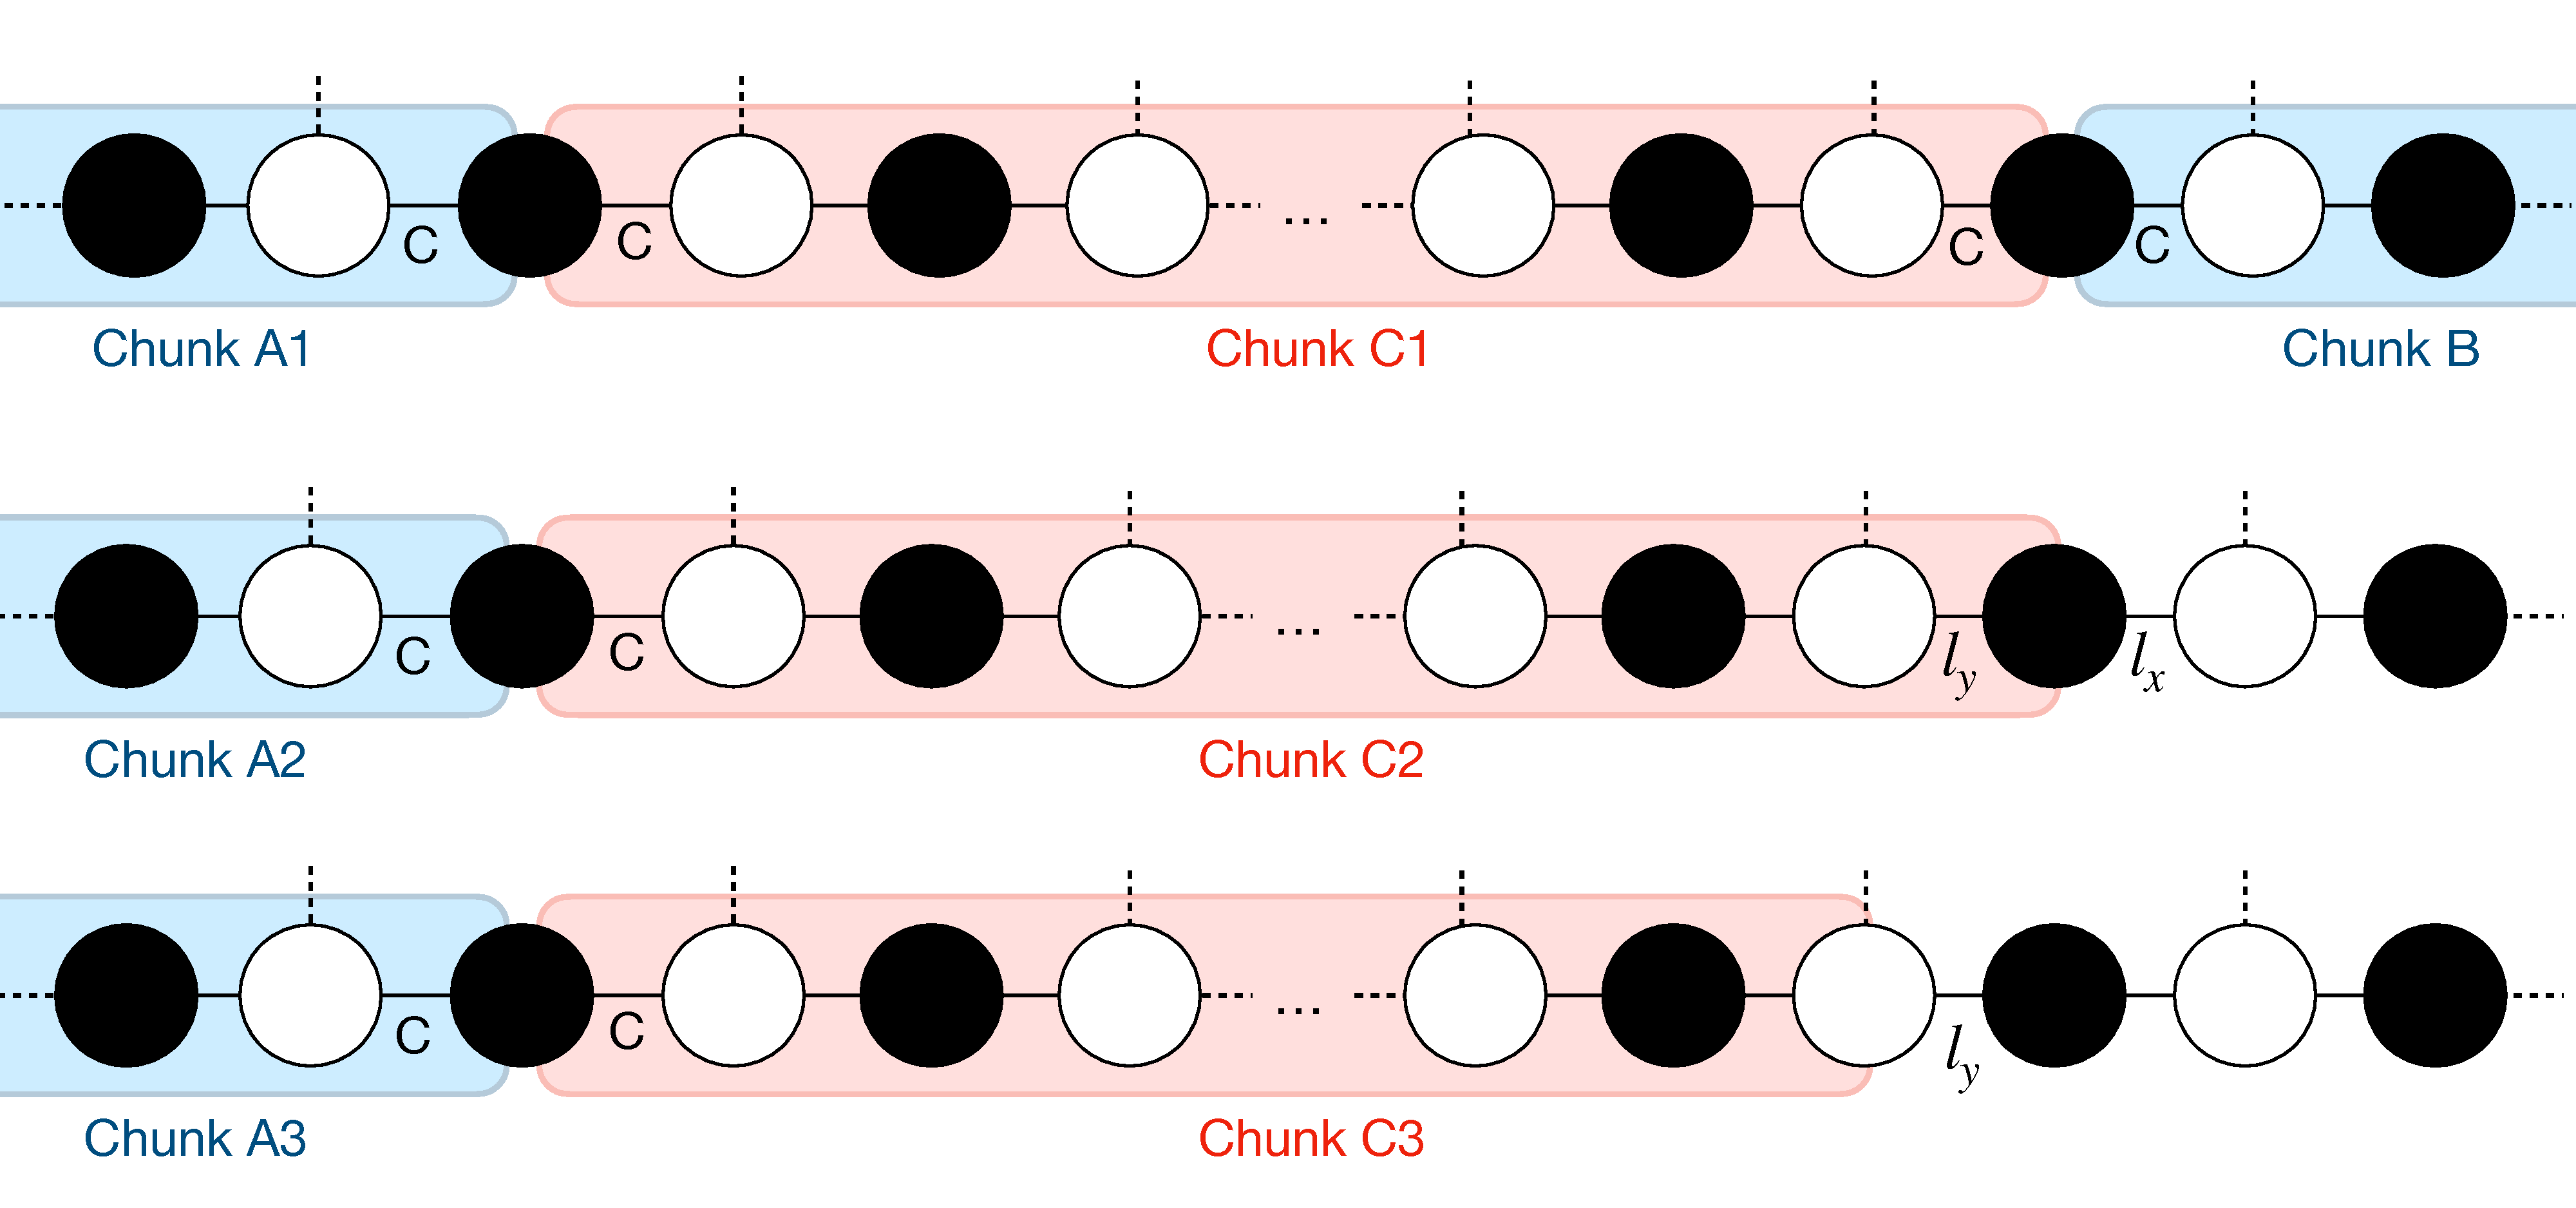
\includegraphics[scale = 0.22]{Figures/graph_rc.pdf}
    \caption{The 3 different chunk's endpoints possibilities}
    \label{fig:global_1}
\end{figure}
Because the chunk's length is at most $c = \mathcal{O}(1)$, we are now going to prove that for each concerned problems, a proper coloring is possible by starting from an endpoint and labelling the path by going through it in constant time.
\end{itemize}
\begin{defi}
(Path labelling). Given a problem $\Pi=(3,2,W,B)$ a path labelling $P(n)$ is a regular expression using the labels of $\Sigma$ that represent exactly 1 string of length $n$. It must respect the following:
\begin{itemize}
    \item For $i=2k, k\in\mathbf{N}$ we have $(P_iP_{i+1})\in B$
    \item For $i=2k+1, k\in\mathbf{N}$ we have $(P_iP_{i+1}X)\in W$ for some $X\in \Sigma$
\end{itemize}
\end{defi}

\begin{claim}
\textit{A chunk of length $n$ whose first edge is $X_1X_2\in B$ and its last edge is $Y_1Y_2\in B$ can be properly labelled in time $\mathcal{O}(1)$ given a path labelling $P(n+1)$ where $(P_0P_1)=X_1X_2$ and $(P_{n-1}P_n)=Y_1Y_2$}\\\\
\textit{Proof.} We start from
\end{claim}

\begin{itemize}
    \item $W=\{ABC\}$
    Let be $k$ the number of black nodes in the chunks excluding both endpoints.
    Let be $CC$ the left endpoint:
    \begin{itemize}
        \item If the right endpoint is $CC$, we can use the path labelling $CC(AB)^kCC$; See the chunk Y1 in .
        \item If the right endpoint is $BA$, we can use the path labelling $CC(BA)^kBA$; See the chunk Y2 in .
        \item If the right endpoint is $AB$, we can use the path labelling $CC(AB)^kAB$; See the chunk Y3 in .
    \end{itemize}
    \item $W=\{ACX_1,BCC\}$ with $X_1\in \Sigma$
    Let be $k$ the number of black nodes in the chunks excluding both endpoints.
    Let be $CC$ the left endpoint:
    \begin{itemize}
        \item If the right endpoint is $CC$, we can use the path labelling $CC(CC)^kCC$; See the chunk Y1 in .
        \item If the right endpoint is $BA$, we can use the path labelling $CC(CC)^kBA$; See the chunk Y2 in .
        \item If the right endpoint is $AB$, we can use the path labelling $CC(CC)^kAB$; See the chunk Y3 in .
    \end{itemize}
    \begin{figure}[htb]
    \centering
    \includegraphics[scale = 0.22]{Figures/graph_rc_2.pdf}
    \caption{The 3 different chunk's endpoints possibilities}
    \label{fig:global_1}
\end{figure}
\end{itemize}

